\section{Moving Beyond Flat Index Tags}
\label{sec:background}

%\begin{figure}[t!] 
%\begin{minipage}{1\linewidth}
%\begin{subfigure}[c]{0.96\linewidth}
%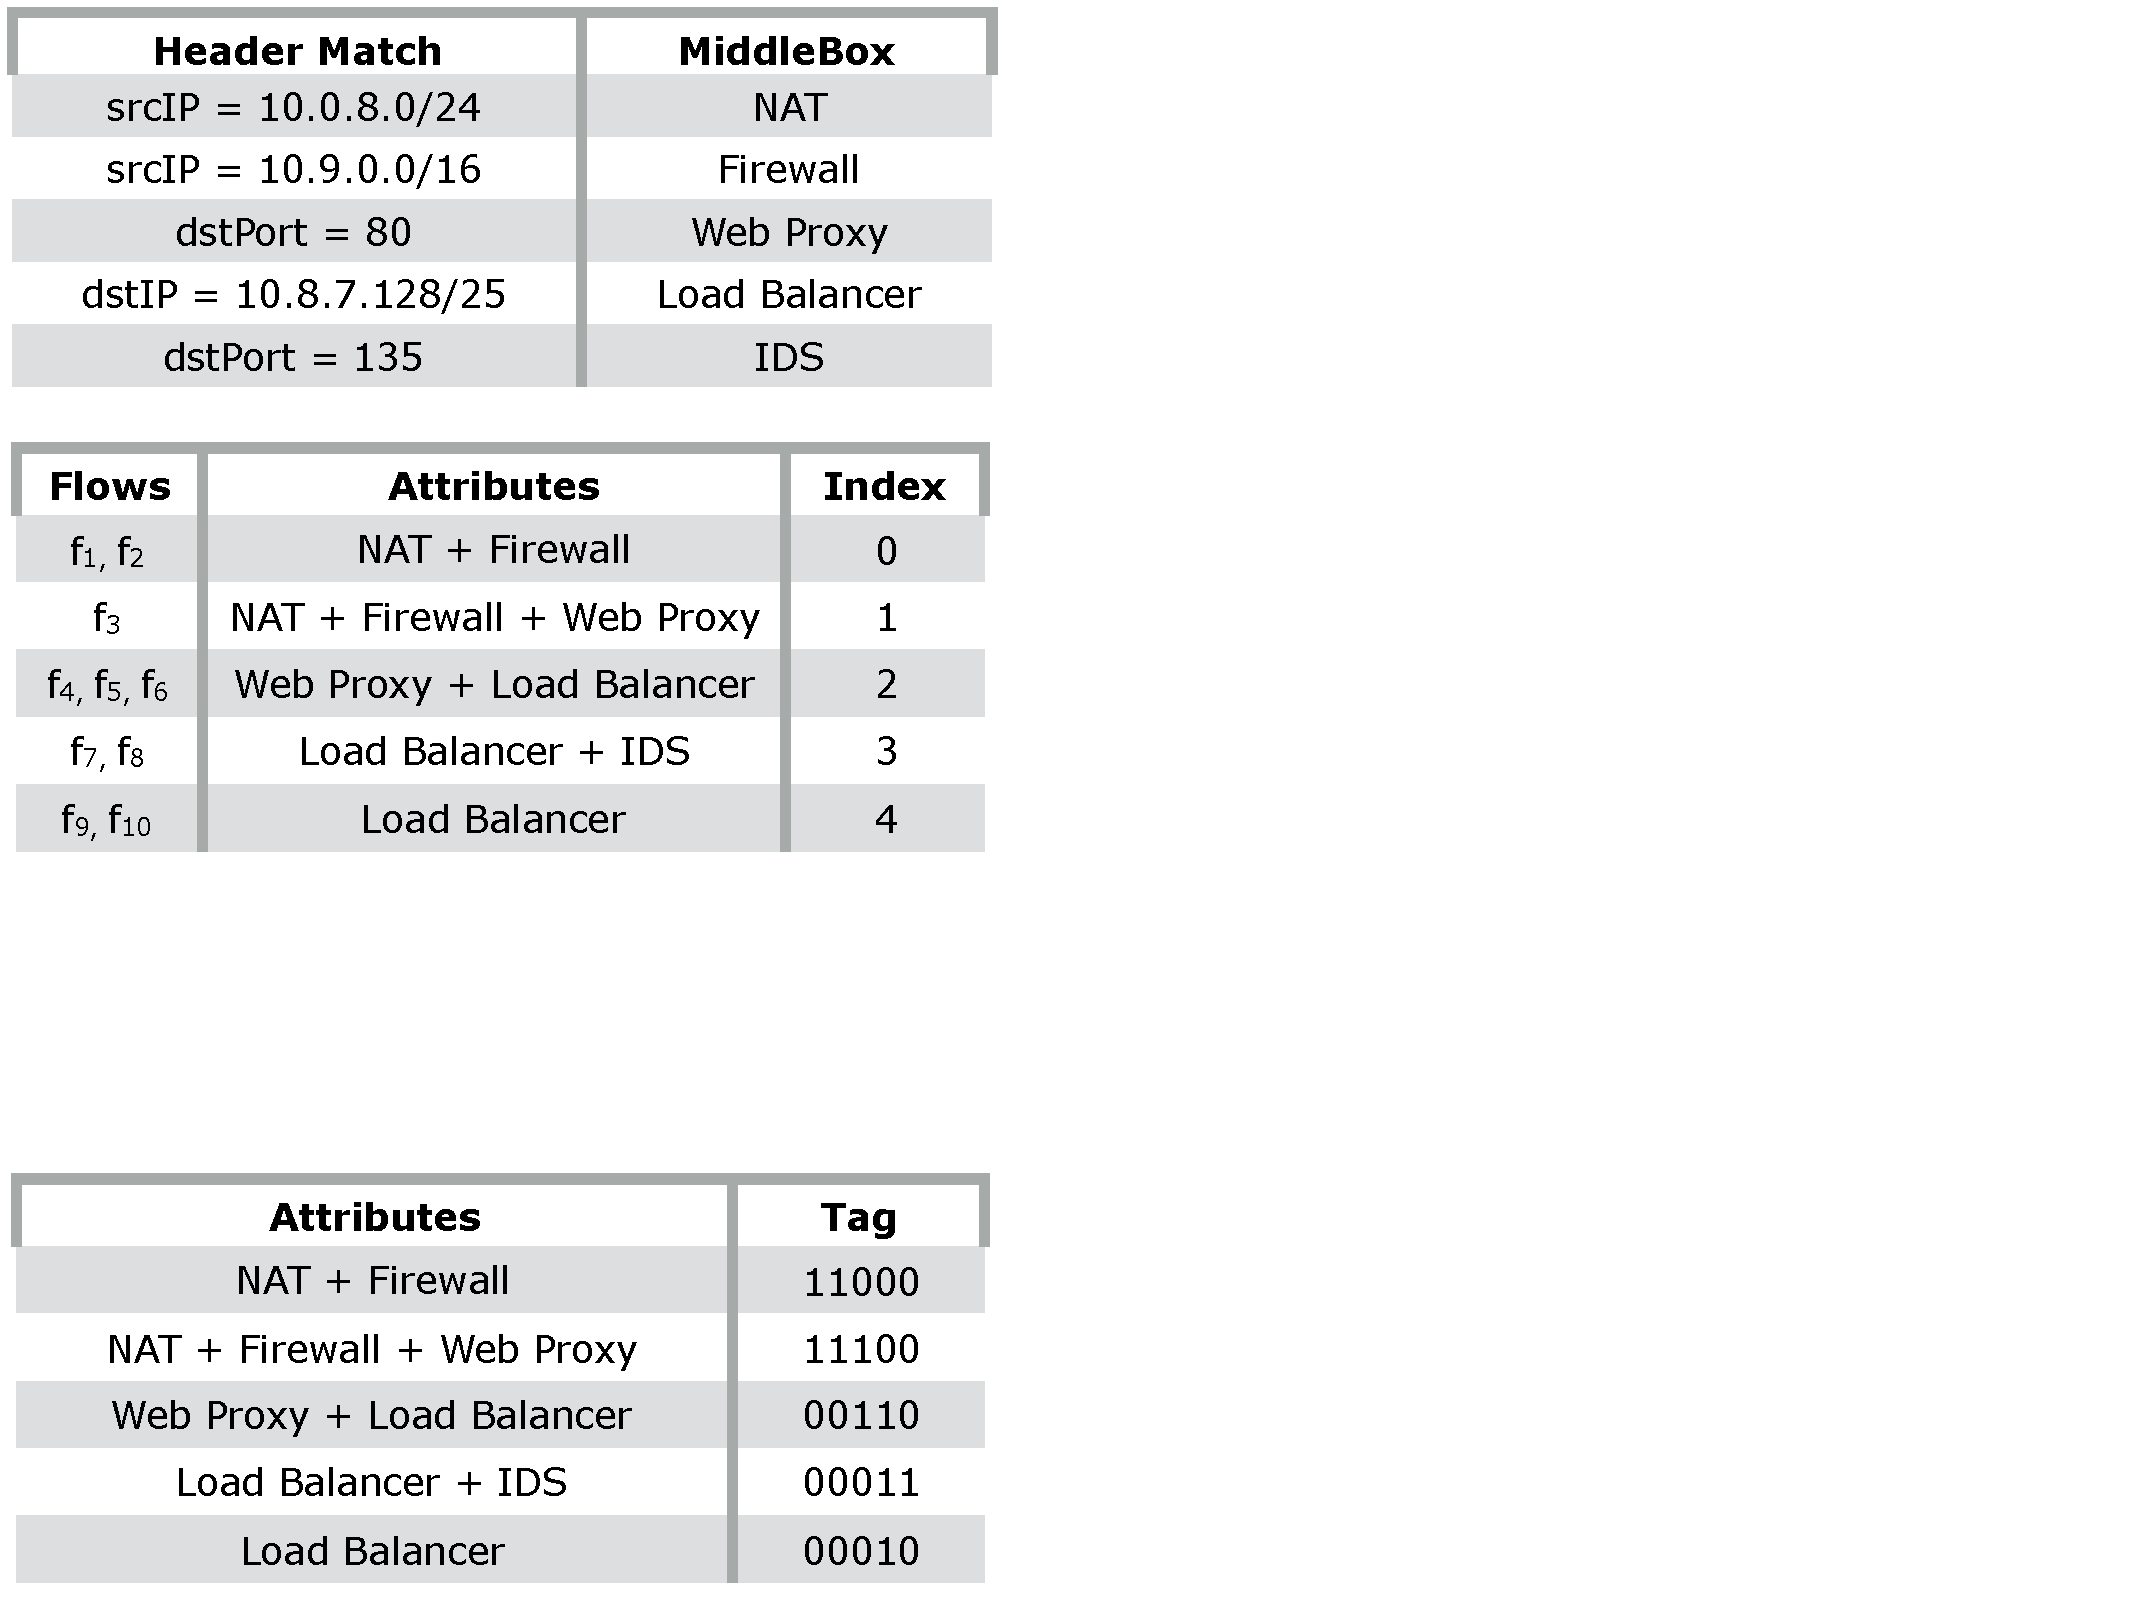
\includegraphics[trim={0 12cm 19cm 0}, clip, width=\linewidth]{figures/mbox_path_example3}
%\end{subfigure} 
%\end{minipage} 
%\caption{In this example, we have a policy that defines traffic which must flow through subsets of five middleboxes. The first table shows which header fields trigger each middlebox, and the second table shows some combinations we may see in network traffic. }
%\label{fig:mbox_policies}
%\end{figure}

Packet labeling schemes need to work within the capabilities of commodity switches.  In this section, we first review packet processing in high-speed switches and how the ``match-action'' capabilities have evolved in recent years.  Next, we discuss flat index tagging and its limitations, and then present several example applications that would benefit from more flexible tagging schemes.

\subsection{Flexible Tags using Flexible Switches}
Commodity switches traditionally use \emph{match-action tables} to determine how to handle packets, based on \textit{forwarding rules} installed at runtime. A table entry consists of a set of match conditions, and an action to take if the matching conditions are met. Actions include dropping a packet, rewriting a header field, or forwarding the packet out a specific port. 
Each matching condition compares a string $S$ to a specific packet header field $H$, using one of three kinds of comparisons:

\begin{itemize}
  \item \textbf{Exact Matching:} $S$ is a binary string, and the match returns true if $S = H$.
  \item \textbf{Longest-Prefix Matching:} $S$ is a ternary string, where the first $x$ characters are binary, and the remaining are the wildcard character $*$. A header field is a match if the $x$ binary characters of $S$ are a prefix of $H$, and there is no other $S'$ in the table which is a longer prefix of $H$. 
  \item \textbf{Wildcard Matching:} $S$ is a ternary string with characters $\{0,1,*\}$ and an associated priority. $S$ matches $H$ if the only characters on which they are unequal are wildcards, and there is no other $S$ in the table which also matches but has a higher priority.
\end{itemize}
  
Until recently, switches imposed significant restrictions on the matching type.  For the vast majority of fields, only exact matching was supported, with the exception of longest-prefix matching for IP addresses. This prevents most fields from being repurposed for anything other than flat tags. However, with recent changes to commodity switches, such as new features supported by OpenFlow 1.3 switches~\cite{of13} and flexible protocol-independent switches~\cite{P4}, we can apply longest-prefix or wildcard matching to existing fields, or even add new fields. Prefix and wildcard matching allows us to treat a header field as a \emph{set} of information, rather than just a single value. 


\begin{figure}[t!] 
\begin{minipage}{1\linewidth}
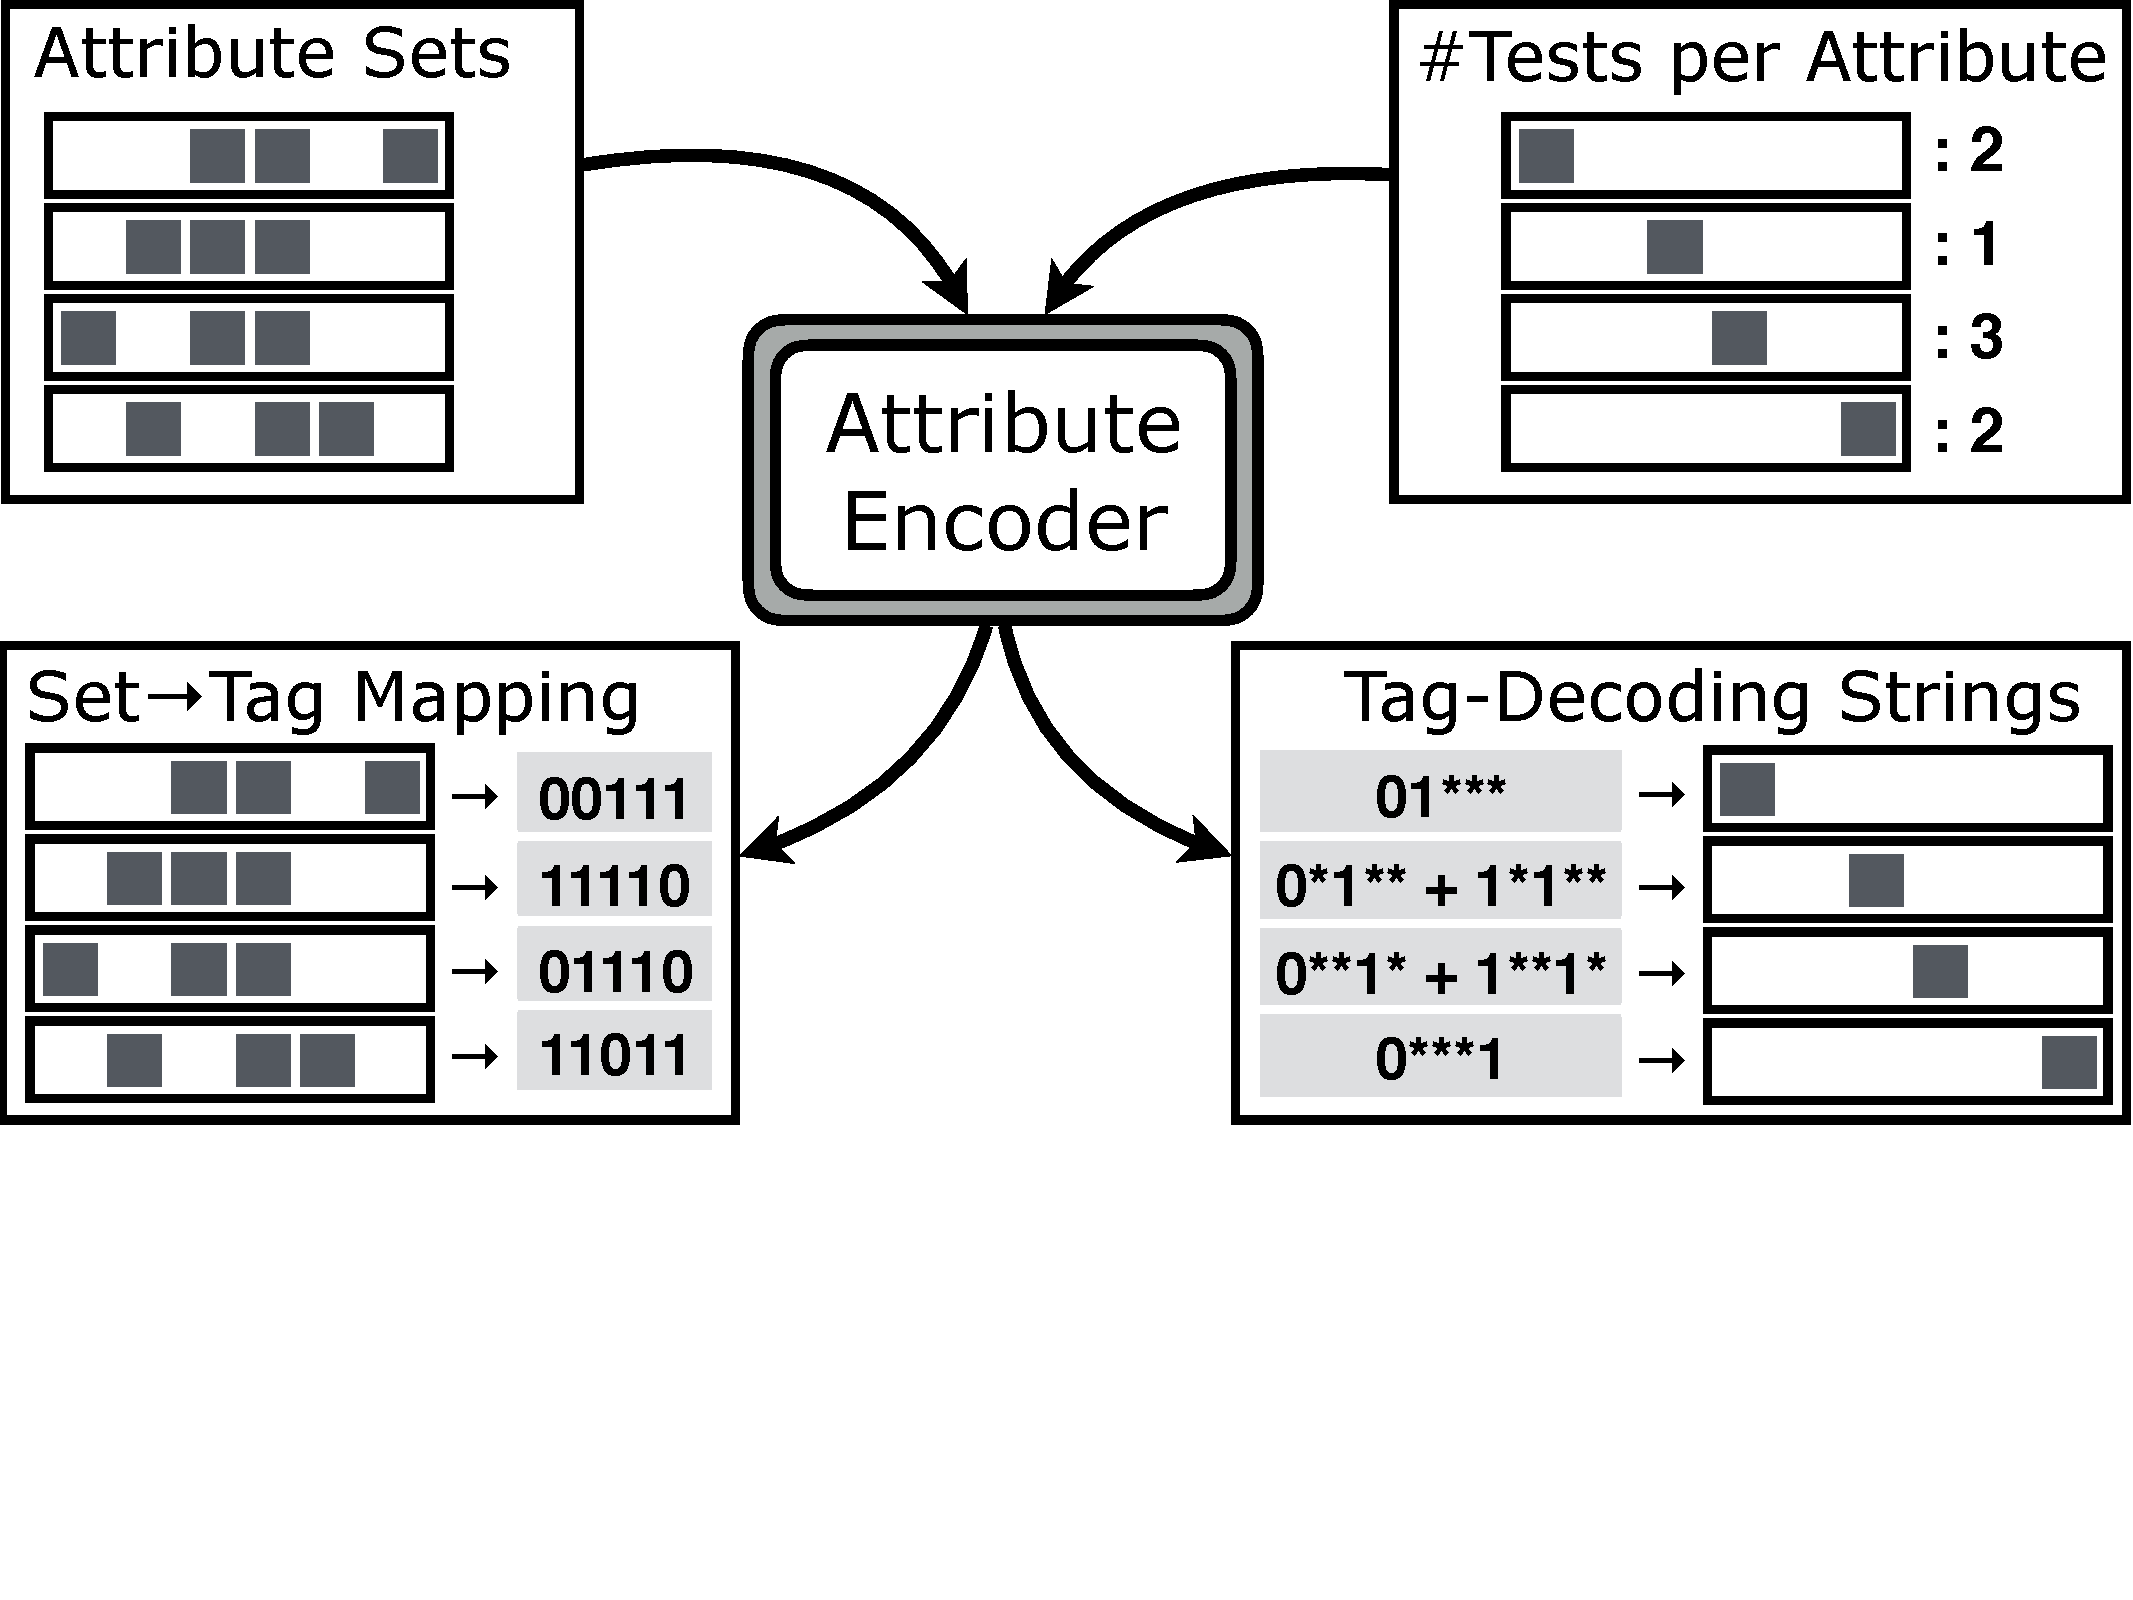
\includegraphics[trim={0 4cm 0 0}, clip, width=\linewidth]{figures/system_flow2}
\end{minipage} 
\caption{An illustration of the information flow for an attribute-encoding tagging scheme. The encoding scheme takes as input a list of attribute sets and the number of queries that will be performed per attribute. The output is a list of tags corresponding to those attribute sets, and wildcard strings used for querying each attribute.}
\label{fig:system_flow}
\end{figure}


